\documentclass{amsart}
\usepackage{amsmath}
\usepackage{amssymb}
\usepackage{proof}
\usepackage{cancel}
\usepackage[usenames,dvipsnames]{color}
\usepackage{graphics}
\usepackage{verbatim}
\usepackage{tikz}

\usetikzlibrary{arrows}

\usepackage{ulem}
\usepackage{caption}

\theoremstyle{definition}

\newtheorem{thm}{Theorem}[section]
\newtheorem{cor}[thm]{Corollary}
\newtheorem{lem}[thm]{Lemma}
\newtheorem{conjecture}[thm]{Conjecture}
\newtheorem{definition}[thm]{Definition}
\newtheorem{proposition}[thm]{Proposition}
\newtheorem{example}[thm]{Example}

\newcommand{\truls}[1]{\textbf{\textcolor{magenta}{(T: #1)}}}
\newcommand{\sjur}[1]{\textbf{\textcolor{blue}{(S: #1)}}}
\newcommand{\piotr}[1]{\textbf{\textcolor{OliveGreen}{(P: #1)}}}
\newcommand{\erik}[1]{\textbf{\textcolor{Peach}{(E: #1)}}}
\newcommand{\todo}[1]{\textcolor{Red}{\footnote{TODO: #1}}}

\newcommand{\nn}{\mathbb N}
\newcommand{\rr}{\mathbb R}
\newcommand{\ca}{\mathcal A}
\newcommand{\cb}{\mathcal B}

% how about some consistent conventions?
\newcommand{\cat}[1]{\mathbf{#1}}

\begin{document}

\section{Background and history}
\begin{description}
\item[Abstract systems] (Emmy Noether)

\begin{quote}
Amalie Emmy Noether (German: [ˈnøːtɐ]; 23 March 1882 – 14 April 1935), sometimes referred to as Emily[1] or Emmy, was an influential German mathematician known for her groundbreaking contributions to abstract algebra and theoretical physics. Described by Pavel Alexandrov, Albert Einstein, Jean Dieudonné, Hermann Weyl, Norbert Wiener and others as the most important woman in the history of mathematics,[2][3] she revolutionized the theories of rings, fields, and algebras. In physics, Noether's theorem explains the fundamental connection between symmetry and conservation laws.[4] (wikipedia)\end{quote}

\item[Universal Algebra] Garrett Birkhoff
\begin{quote}
Garrett Birkhoff (January 19, 1911 – November 22, 1996) was an American mathematician. He is best known for his work in lattice theory. (wikipedia)
\end{quote}

\begin{quote}The following paper is a study of abstract algebras qua abstract algebras. As no vocabulary suitable for this purpose is current, I have been forced to use a number of new terms, and extend the meaning of some accepted ones. (abstract, ``On the structure of Abstract Algebra'' 1935)
\end{quote}
\end{description}

\section{Mathematical Preliminaries}

\begin{definition}\textbf{(Stream)} A \textit{stream} $(S, \leq)$ over alphabet $A$ is a subset of lists over $A$, $S \subseteq A^\ast$ together with an ordering $\leq$ such that
\begin{itemize}
\item $(S, \leq)$ is linearly ordered, and
\item $(S, \leq)$ is prefix closed.
\end{itemize}
\end{definition}

\begin{definition}\textbf{(Infinite Tree)} An \textit{infinite tree} is like a stream, but not linearly ordered.
\end{definition}

\begin{definition}\textbf{(Algebra)} An \textit{algebra} is a tuple $(C, op_1, \dots, op_n)$ where
\begin{itemize}
\item $C$ is a non-empty set called the \textit{carrier set}, and
\item for each $1 \leq i \leq n$, $op_i : C^x \to C$.
\end{itemize}
\end{definition}

\begin{definition}\textbf{(Signature)} A \textit{signature} is a pair $\Sigma = (OP, ar)$ where
\begin{itemize}
\item $OP$ is a set of operation names, and
\item $ar : OP \to \mathbb N$ is the arity map.
\end{itemize}
\end{definition}

\begin{example} Here are some algebras.
  \begin{enumerate}
  \item $\mathcal N_1$ is an algebra with carrier set $\mathbb N$ and a single operation $s : \nn \to \nn$.
  \item $\mathcal N_2$ is an algebra with carrier set $\nn$ and two operations: $s : \nn \to \nn$ and $\_+\_ : \nn \times \nn \to \nn$.
  \item $\mathcal R_\ast$ is an algebra where the carrier set is the set of positive real numbers $\mathbb R_+$ and the three operations are the constant $1 : \rr_+^0 \to \rr_+$ (or $1 : \mathbf 1 \to \rr_+$), the unary map $\frac 1 \_ : \rr_+ \to \rr_+$, and the binary operation $\_*\_ : \rr_+^2 \to \rr_+$.
  \item $\mathcal L$ is a \textit{two-sorted} algebra (of lists) where the carriers are $\nn$ and $\nn^\ast$, the operations are
    \begin{itemize}
    \item a constant (empty list) $[\ ] : \mathbf 1 \to \nn^\ast$,
    \item binary (building) $\_ :\_ : \nn \times \nn^\ast \to \nn^\ast$, and
    \item binary (concatination) $\_ ++ \_ : \nn^\ast \times \nn^\ast \to \nn^\ast$.
    \end{itemize}
  \item $\wp$ is a two-sorted algebra where the carrier sets are $\nn$ and $\wp \nn$, with operations
    \begin{itemize}
    \item constant $\emptyset : \mathbf 1 \to \wp \nn$,
    \item binary $\{\_\}\cup\_ : \nn \times \wp \nn \to \wp \nn$, and
    \item binary $\_ \cup \_ : \wp\nn \times \wp \nn \to \wp \nn$.
    \end{itemize}
  \end{enumerate}

  Here is a signature.
  \begin{enumerate}
    \item $\Sigma_1 = (OP_1, ar_1)$ where $OP_1 = \{c, u\}$, $ar_1(c) = 0$ and $ar_1(u) = 1$. 

      (The signature of a simple algebra with one constant and one unary operation.)
  \end{enumerate}
\end{example}

\begin{definition}\textbf{(Subalgebra)} An $\Sigma$-algebra $\ca$ is a subalgebra of $\Sigma$-algebra $\cb$ if
\begin{itemize}
\item $A \subseteq B$, and
\item $op^\ca = op^\cb \downarrow A^{ar(op)}$ for each $op \in OP$.
\end{itemize}
\end{definition}

If $\ca$ is a subalgebra of $\cb$, $A$ contains all constants and $A$ is closed under the operations in $\cb$.

\begin{definition}\textbf{(Homomorphism)} $f : \ca \to \cb$ is a \textit{$\Sigma$-homomorphism} from $\ca$ to $\cb$ if
\begin{itemize}
\item $f : A \to B$, and 
\item for all $op \in OP$ and all $(a_1, \dots, a_n) \in A^{ar(op)}$
$$f(op^\ca(a_1, \dots, a_n)) = op^\cb(f(a_1), \dots, f(a_n)).$$
\end{itemize}
or, more diagramatically, the following diagram commutes

\begin{center}
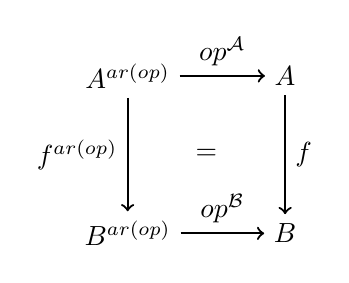
\begin{tikzpicture}
\node (srcA) at (0.0, 2.0) {$A^{ar(op)}$};
\node (trgA) at (2.0, 2.0) {$A$};
\node (srcB) at (0.0, 0.0) {$B^{ar(op)}$};
\node (trgB) at (2.0, 0.0) {$B$};

\node (eq) at (1.0, 1.0) {$=$};

\tikzset{mystyle/.style={->,thick}};  
\path (srcA) edge [mystyle] node[above]{$op^\ca$} (trgA);
\path (srcB) edge [mystyle] node[above]{$op^\cb$} (trgB);
\path (srcA) edge [mystyle] node[left]{$f^{ar(op)}$} (srcB);
\path (trgA) edge [mystyle] node[right]{$f$} (trgB);
\end{tikzpicture}
\end{center}
\end{definition}

\begin{proposition} A $\Sigma$-homomorphism $f : \ca \to \cb$ is
\begin{description}
\item [monic] iff $f : A \to B$ is \textit{injective}
\begin{center}
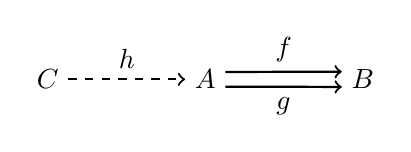
\begin{tikzpicture}
\node (A) at (-1.0, 0.0) {$A$};
\node (B) at (1.0, 0.0) {$B$};
\node (C) at (-3, 0) {$C$};

\tikzset{mystyle/.style={->,thick}};  
\path (A.20) edge [mystyle] node[above]{$f$} (B.160);
\path (A.340) edge [mystyle] node[below]{$g$} (B.200);
\tikzset{mystyle/.style={->,thick,dashed}};  
\path (C) edge[mystyle] node[above]{$h$} (A);
\end{tikzpicture}
\end{center}

\item [epic] iff $f : A \to B$ is \textit{surjective}
\begin{center}
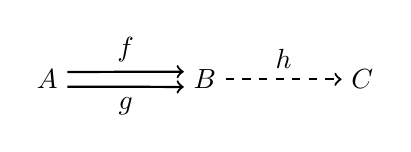
\begin{tikzpicture}
\node (A) at (-1.0, 0.0) {$A$};
\node (B) at (1.0, 0.0) {$B$};
\node (C) at (3, 0) {$C$};

\tikzset{mystyle/.style={->,thick}};  
\path (A.20) edge [mystyle] node[above]{$f$} (B.160);
\path (A.340) edge [mystyle] node[below]{$g$} (B.200);
\tikzset{mystyle/.style={->,thick,dashed}};  
\path (B) edge[mystyle] node[above]{$h$} (C);
\end{tikzpicture}
\end{center}

\item [iso] iff $f : A \to B$ is \textit{bijective}
\begin{center}
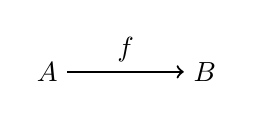
\begin{tikzpicture}
\node (A) at (-1.0, 0.0) {$A$};
\node (B) at (1.0, 0.0) {$B$};

\tikzset{mystyle/.style={->,thick}};  
\path (A) edge [mystyle] node[above]{$f$} (B);
\end{tikzpicture}
\end{center}
\end{description}
\end{proposition}

\subsection{Epi-mono factorization and the kernel}
For any map $f : A \to B$ there is an epi-mono factorization. That is there are maps $f'_1 : A \to Z$ and $f'_2 : Z \to B$ such that 
\begin{itemize}
\item $f'_1$ is epi, 
\item $f'_2$ is mono, and
\item $f = f'_1;f'_2$.
\end{itemize}

\begin{proposition} Epi-mono factorizations are unique upto isomorphisms
\begin{center}
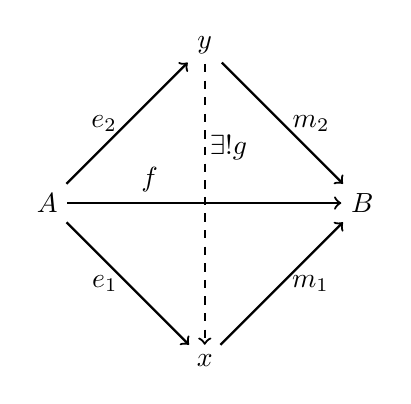
\begin{tikzpicture}
\node (A) at (-2.0, 0.0) {$A$};
\node (B) at (2.0, 0.0) {$B$};

\node (y) at (0, 2) {$y$};
\node (x) at (0, -2) {$x$};

\node (f) at (-0.7, 0.3) {$f$};
\node (g) at (0.3, 0.7) {$\exists ! g$};

\tikzset{mystyle/.style={->,thick}};  
\path (A) edge [mystyle] node {} (B);
\path (A) edge[mystyle] node[left]{$e_2$} (y);
\path (A) edge[mystyle] node[left]{$e_1$} (x);
\path (y) edge[mystyle] node[right]{$m_2$} (B);
\path (x) edge[mystyle] node[right]{$m_1$} (B);
\tikzset{mystyle/.style={->,thick,dashed}};  
\path (y) edge[mystyle] node[right]{} (x);
\end{tikzpicture}
\end{center}
\end{proposition}

\begin{definition}\textbf{(Kernel)} The \textit{kernel} $ker(f)$ of a function is the relation
$$ker(f) = \{(a,a') \in A \times A ~|~ f(a) = f(a')\}$$
\end{definition}

The kernel of a function induces an equivalence on the domain
\begin{equation} 
\equiv ~:=~ ker(f)
\end{equation}

This allows the construction of the quotient set 
\begin{equation}
A/_\equiv ~:=~ \{[a]_\equiv ~|~ a \in A\} \text{ where } [a]_\equiv = \{a' ~|~ (a,a') \in \equiv\}
\end{equation}

\begin{center}
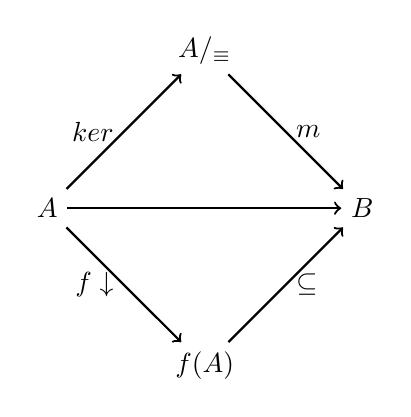
\begin{tikzpicture}
\node (A) at (-2.0, 0.0) {$A$};
\node (B) at (2.0, 0.0) {$B$};

\node (y) at (0, 2) {$A/_\equiv$};
\node (x) at (0, -2) {$f(A)$};

\tikzset{mystyle/.style={->,thick}};  
\path (A) edge [mystyle] node {} (B);
\path (A) edge[mystyle] node[left]{$ker$} (y);
\path (A) edge[mystyle] node[left]{$f\downarrow$} (x);
\path (y) edge[mystyle] node[right]{$m$} (B);
\path (x) edge[mystyle] node[right]{$\subseteq$} (B);
\end{tikzpicture}
\end{center}

\begin{definition}\textbf{(Equ(A))} All equivalence classes on $A$ is $Equ(A)$. 
\end{definition}

\begin{proposition} About $Equ(A)$
\begin{itemize}
\item $Equ(A)$ is ordered by $\subseteq$
\begin{itemize}
\item the minimal element is the diagonal $\Delta_A = \{(a,a) ~|~ a \in A\}$
\item the maximal element is the complete graph $A\times A$
\end{itemize}
\item \textbf{meet:} Equ(A) is closed under intersection
\item \textbf{join:} the join of $\equiv_1$ and $\equiv_2$ is the equivalence class $\equiv$ generated by $\equiv_1 \cup \equiv_2$.
\end{itemize}
\end{proposition}

\begin{definition}\textbf{($\Sigma$-conguence)} Let $\ca$ be an algebra. $\equiv ~\subseteq~ A^2$ is a $\Sigma$-congruence if
\begin{itemize}
\item $\equiv$ is an equivalence relation on $A$, and 
\item for each $op \in OP$ with $n = ar(op)$
$$ \text{if } (a_1, a_1'), \dots , (a_n, a_n') \in \equiv \text{ then } (op^\ca(a_1, \dots, a_n), op^\ca(a_1', \dots, a_n')) \in \equiv$$
\end{itemize}
\end{definition}

\begin{proposition} if $f$ is a $\Sigma$-homomorphism, then $ker(f)$ is a $\Sigma$-congruence.
\end{proposition}

Categorically, the kernel is an equalizer of $\pi_1;f$ and $\pi_2;f$ (i.e., a pullback of $(f,f)$) in the following diagram
\begin{center}
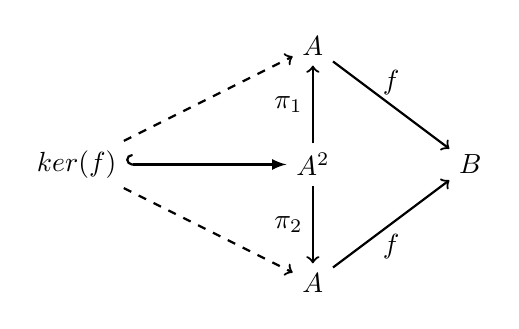
\begin{tikzpicture}
\node (A) at (0.0, -1.5) {$A$};
\node (A') at (0, 1.5) {$A$};
\node (A2) at (0, 0) {$A^2$};

\node (B) at (2.0, 0.0) {$B$};
\node (ker)  at (-3, 0) {$ker(f)$};


\tikzset{mystyle/.style={->,thick}};  
\path (A) edge [mystyle] node[below]{$f$} (B);
\path (A') edge [mystyle] node[above]{$f$} (B);
\path (A2) edge[mystyle] node[left]{$\pi_2$} (A);
\path (A2) edge[mystyle] node[left]{$\pi_1$} (A');
\tikzset{mystyle/.style={->,thick,dashed}};  
\path (ker) edge[mystyle] node{} (A);
\path (ker) edge[mystyle] node{} (A');
\tikzset{mystyle/.style={->,thick,right hook-latex}};  
\path (ker) edge[mystyle] node[above]{} (A2);
\end{tikzpicture}
\end{center}

\truls{Do we need more on kernels and category theory?}

\piotr{Not sure, but pasting notes from my talk here anyway}

\section{Piotr's take on Basic Constructions}

\subsection{What is a category?}

A \emph{category} $\mathbf{C}$ is a tuple comprising of:

\begin{enumerate}
\item a collection of \emph{objects};
\item a collection of \emph{morphisms} or \emph{arrows};
\item  operations assigning to each morphism $f$ a \emph{domain} $dom\ f$,
  and a \emph{codomain} $cod\ f$. We write $f: A \to B$ to show that
  $dom\ f = A$ and $cod\ f = B$. The collection of all arrows with
  domain $A$ and codomain $B$ is written $\mathbf{C}(A,B)$.
\item a composition operator assigning to each pair of arrows $f$ and $g$ a
  \emph{composite arrow} $g\circ f: dom\ f\to cod\ g$ that satisfies the
  law of associativity, i.e.~for any arrows $f: A \to B$, $g: B\to C$
  and $h: C \to D$: \[
  h\circ (g \circ f) = (h \circ g) \circ f
  \]
\item for each object $A$, an \emph{identity} arrow $id_A: A \to A$ that
  satisfies the identity law, i.e.~for any arrow $f: A\to B$:
  $id_B \circ f = f$ and $f\circ id_A = f$
\end{enumerate}

\textbf{Remark:} Collections mentioned above are meant in a
set-theoretical sense, i.e.~they are just sets or proper classes.

First we present a simple example, describing the category of sets.

\subsubsection{Example: $\mathbf{Set}$}

\begin{enumerate}
\item Objects in $\mathbf{Set}$ are sets.
\item Arrows $f: A\to B$ are total functions from set $A$ into set $B$.
\item For every total function $f$, its domain $A$ and codomain $B$, we get
  $dom\ f = A$, $cod\ f = B$, and $f \in \mathbf{Set}(A, B)$.
\item Composition of one total function $f: A\to B$ with another total
  function $g: B\to C$ is the total function from $A$ to $C$ mapping
  each element $a \in A$ to $g(f(a))\in C$. Composition of total
  functions on sets is associative: for any $f: A\to B$, $g: B\to C$ and
  $h:C \to D$, we get $h\circ (g\circ f) = (h\circ g)\circ f$.
\item For each set $A$, the identity function $id_A$ is a total function
  with domain and codomain $A$. For any function $f: A\to B$, the
  identity functions on $A$ and $B$ satisfy the equations required by
  the identity law: $id_B \circ f = f$ and $f \circ id_A = f$.
\end{enumerate}

\subsection{Dual notions}

For each category $\cat{C}$, the objects of the dual category $\cat{C}^{op}$ are the same as those in $\cat{C}$, but the arrows in $\cat{C}^{op}$ are opposite. If $f: A~\to B$ is an arrow of $\cat{C}$ then $f: B \to A$ is an arrow of $\cat{C}^{op}$. 

\subsubsection{Duality of injective \& surjective functions}

\begin{definition}
An arrow $f: B \to C$ is \emph{monic} if, for any pair of arrows $g: A\to B$ and $h: A\to B$, $g;\! f = h;\! f$\footnote{Not sure how to write compositions, which convention to follow. } implies $g=h$.
\end{definition}

\begin{proposition}
In $\cat{Set}$, monic arrows are just the injective functions ($f(x) = f(x)$ implies $x=y$). 
\end{proposition}

\begin{proof}
  Let $f: B\to C$ be an injective function, and let $g,h: A\to B$ be such that $g;\! f = h;\! f$, but $g\neq h$. This means there is an element $a\in A$ for which $g(a) \neq h(a)$. But since $f$ is injective, $f(g(a))\neq f(h(a))$ which contradicts $g;\! f = h;\! f$. So $f$ is monic.

  Conversely, let $f: B \to C$ be monic. If it's not injective, there are distinct elements $b, b' \in B$ for which $f(b) = f(b')$. Let $A$ be a~singleton set $\{a\}$, and let $g: A\to B$ map $a$ to $b$ while $h: A\to B$ maps $a$ to $b'$. Then $f(g(a)) = f(h(a))$, contradicting the assumption that $f$ is monic. 
\end{proof}

\begin{definition}
An arrow $f: A\to B$ is \emph{epic} if, for any pairs of arrows $g: B\to C$ and $h: B\to C$, $f;\! g = f;\! h$ implies $g=h$. Epic is clearly dual to monic. 
\end{definition}

\begin{proposition}
In $\cat{Set}$, epic arrows are just the surjective functions. 
\end{proposition}

\begin{proof}
  nigga please
\end{proof}

\subsubsection{Empty \& singleton sets}

\begin{definition}
An object is called \emph{initial} if, for every object in $A$, there is exactly one arrow from it to $A$. 
\end{definition}

\begin{definition}
Dually, an object is \emph{terminal} if, for every object in $A$, there is exactly one arrow from $A$ to $1$. 
\end{definition}

In $\cat{Set}$, the empty set $\emptyset$ is the only initial object: for every set $S$, the empty function is the only function from $\emptyset$ to $S$.

Dually, each singleton set is a~terminal object, since for every set $S$ there is a~function from $S$ to a~singleton set $\{x\}$ mapping every element of $S$ to $x$, and this is the only total function from $S$ to $\{x\}$. 

\subsubsection{Cartesian products and disjoint unions}

\begin{itemize}
\item elements can be treated as arrows from a~terminal object
\item when we form a~product $A\times B$ we also define projections $\pi_{1}: A\times B \to A$ and $\pi_{2}: A\times B \to B$
\item so product is actually a~tuple $(A\times B, \pi_{1},\pi_{2})$.
\end{itemize}

Let $C$ be a~set and $f: C\to A$, $g: C\to B$. We say a~\emph{product function} $\langle f,g\rangle: C \to A\times B$ is
\[
\langle f, g\rangle (x) = (f(x), g(x))
\]
Functions $f$ and $g$ can be recovered from $\langle f, g\rangle$ by setting $f = \langle f,g\rangle;\! \pi_{1}$ and $g = \langle f, g\rangle;\! \pi_{2}$.

\begin{definition}
  A~\emph{product} of two objects $A$ and $B$ is an object $A\times B$ together with \emph{projection arrows} $\pi_{1}: A\times B \to A$ and $\pi_{2}: A\times B \to B$, such that for any object $C$ and pair of arrows $f: C\to A$ and $g: C\to B$ there is exactly one \emph{mediating} arrow $\langle f,g\rangle: C\to A\times B$ making the diagram
  
  \begin{center}
    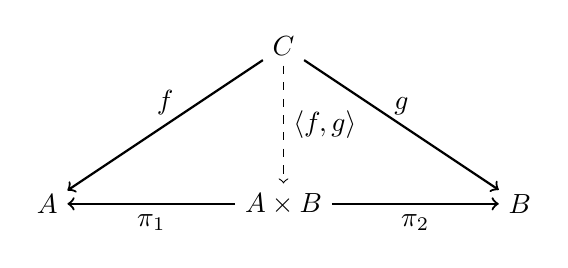
\begin{tikzpicture}
      \node (C)   at (0, 2) {$C$};
      \node (A)   at (-3, 0) {$A$};
      \node (B)   at (3, 0) {$B$};
      \node (AxB) at (0, 0) {$A\times B$};
      
      \tikzset{mystyle/.style={->,thick}};
 
      \path (AxB) edge [mystyle] node[below]{$\pi_{1}$} (A);
      \path (AxB) edge [mystyle] node[below]{$\pi_{2}$} (B);
      
      \path (C) edge[mystyle] node[left,above]{$f$} (A);
      \path (C) edge[mystyle] node[right,above]{$g$} (B);
      \tikzset{mystyle/.style={->,dashed}};
      \path (C) edge [mystyle] node[right]{$\langle f,g\rangle$} (AxB);
    \end{tikzpicture}
  \end{center}
  commute, i.e. $\langle f,g\rangle;\! \pi_{1} = f$ and $\langle f,g\rangle;\! \pi_{2} = g$.
\end{definition}

\begin{definition}
  A~\emph{coproduct} of $A$ and $B$ is $A+B$ together with two \emph{injection arrows} $c_{1}: A\to A+B$, $c_{2}: B \to A+B$, such that for any object $C$ and pair of arrows $f: A\to C$ and $g: B\to C$ there is exactly one arrow $[f,g]: A+B \to C$ making the diagram below commute.
  \begin{center}
    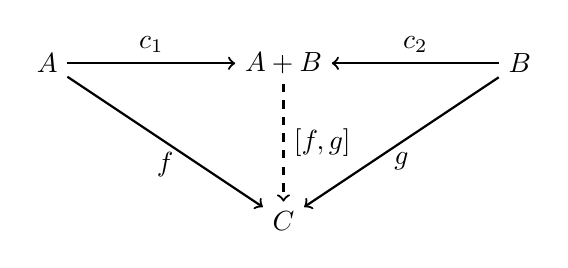
\begin{tikzpicture}
      \node (A)   at (-3, 0) {$A$};
      \node (A+B) at (0,0)   {$A+B$};
      \node (B)   at (3,0)   {$B$};
      \node (C)   at (0,-2)  {$C$};

      \tikzset{mystyle/.style={->,thick}};
      \path (A) edge [mystyle] node[above]{$c_{1}$} (A+B);
      \path (B) edge [mystyle] node[above]{$c_{2}$} (A+B);
      \path (A) edge [mystyle] node[left,below]{$f$} (C);
      \path (B) edge [mystyle] node[right,below]{$g$} (C);

      \tikzset{mystyle/.style={->,thick,dashed}};
      \path (A+B) edge [mystyle] node[right]{$[f,g]$} (C);
    \end{tikzpicture}
  \end{center}
  \emph{Remark:} $[f,g]$ is a~case distinction. 
\end{definition}

\section{Initial $\Sigma$-algebras}
\begin{minipage}[b]{0.4\linewidth}
\begin{center}
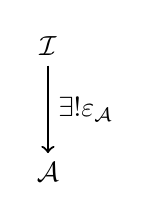
\begin{tikzpicture}
\node (I) at (0.0, 0.8) {$\mathcal I$};
\node (A) at (0.0, -0.8) {$\ca$};

\tikzset{mystyle/.style={->,thick}};  
\path (I) edge [mystyle] node[right]{$\exists!\varepsilon_\ca$} (A);
\end{tikzpicture}
\end{center}
\end{minipage}
\begin{minipage}[b]{0.5\linewidth}
For all $\Sigma$-algebras, there is a unique $\Sigma$-homomorphism, $\varepsilon_\ca : \mathcal I \to \ca$.\\
$\rightsquigarrow~$ \textit{ground term} $\Sigma$-algebra, $\tau_\Sigma$\\
\end{minipage}

\begin{definition}\textbf{(Ground terms)} For a given signature $\Sigma$, the \textit{ground terms} $\tau_\Sigma$ is the least set which satisfies\footnote{Terms (elements of the carrier set of the term algebra) are underlined.}
$$\text{if } \underline{t_1}, \dots, \underline{t_n} \in \tau_\Sigma \text{ and }ar(op) = n \text{ then } \underline{op(t_1, \dots, t_n)} \in \tau_\Sigma.$$
\end{definition}

\begin{definition}\textbf{(Term algebra)} The \textit{term algebra} for a signature $\Sigma$, is the algebra where the carrier set is the set of ground terms, and the operations are defined by
$$op^{\tau_\Sigma}(\underline{t_1}, \dots , \underline{t_n}) ~:=~ \underline{op(t_1, \dots, t_n)}.$$
\end{definition}

Is the term algebra initial? 

\begin{proposition}Yes.
\end{proposition}

\begin{proof} Let $\ca$ be an arbitrary $\Sigma$-algebra.
\begin{center}
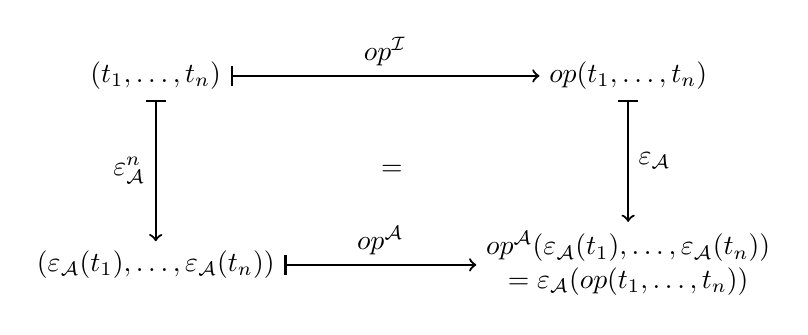
\begin{tikzpicture}
\node (nw) at (-3, 1.2) {$(t_1, \dots, t_n)$};
\node (ne) at (3, 1.2) {$op(t_1, \dots, t_n)$};
\node (sw) at (-3, -1.2) {$(\varepsilon_\ca(t_1), \dots, \varepsilon_\ca(t_n))$};
\node (se) at (3, -1.2) {$\begin{matrix}op^\ca(\varepsilon_\ca(t_1), \dots, \varepsilon_\ca(t_n))\\=\varepsilon_\ca(op(t_1, \dots, t_n))\end{matrix}$};
\node (eq) at (0, 0) {$=$};

\tikzset{mystyle/.style={|->,thick}};  
\path (nw) edge [mystyle] node[left]{$\varepsilon_\ca^n$} (sw);
\path (nw) edge [mystyle] node[above]{$op^{\mathcal I}$} (ne);
\path (ne) edge [mystyle] node[right]{$\varepsilon_\ca$} (se);
\path (sw) edge [mystyle] node[above]{$op^\ca$} (se);
\end{tikzpicture}
\end{center}
\end{proof}

\subsection{Characterization of Initial $\Sigma$-algebras}
\begin{itemize}
\item all $op^{\mathcal I}$ are injective
\item for all $op_1 \neq op_2$
$$op^{\mathcal I}_1(\underbrace{I^{ar(op_1)}}_{(*)}) \cap op^{\mathcal I}_2(\underbrace{I^{ar(op_2)}}_{(*)}) = \emptyset.$$
$(*)$ is a vector of appropriate arguments
\item for all $i \in I$ there exists $op \in OP$ and $i_1, \dots, i_n \in I$ such that
$$ op(i_1, \dots, i_n) = i.$$
\item $\mathcal I$ has no propper subalgebras
\end{itemize}

\section{Induction $\simeq$ Initiality ($\simeq$ Universal property of Constructors)}
\begin{example}Let's define the function $2 * \_ : \nn \to \nn$! 
\begin{description}
\item[Old school] Base case: $2 * 0 := 0$; induction step: $2 * s(n) := (2 * n) + 2$.
\item[21st century] ``Make it communte!'' (Paraphrasing Tom Waits)
\begin{figure}[ht]
\begin{minipage}[b]{0.4\linewidth}
\begin{center}
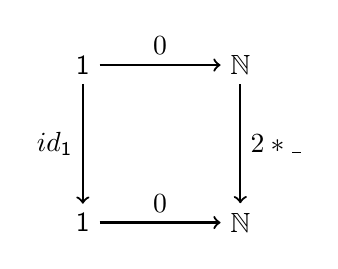
\begin{tikzpicture}
\node (a1) at (-1, 1) {$\mathsf 1$};
\node (a2) at (1, 1) {$\nn$};
\node (b1) at (-1, -1) {$\mathsf 1$};
\node (b2) at (1, -1) {$\nn$};

\tikzset{mystyle/.style={->,thick}};  
\path (a1) edge [mystyle] node[above]{$0$} (a2);
\path (a1) edge [mystyle] node[left]{$id_{\mathsf 1}$} (b1);
\path (b1) edge [mystyle] node[above]{$0$} (b2);
\path (a2) edge [mystyle] node[right]{$2 * \_$} (b2);
\end{tikzpicture}
\end{center}
\caption{\\Base case}
\end{minipage}
\begin{minipage}[b]{0.4\linewidth}
\begin{center}
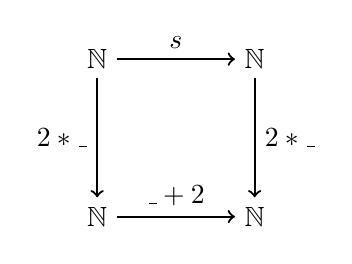
\begin{tikzpicture}
\node (a1) at (-1, 1) {$\nn$};
\node (a2) at (1, 1) {$\nn$};
\node (b1) at (-1, -1) {$\nn$};
\node (b2) at (1, -1) {$\nn$};

\tikzset{mystyle/.style={->,thick}};  
\path (a1) edge [mystyle] node[above]{$s$} (a2);
\path (a1) edge [mystyle] node[left]{$2 * \_$} (b1);
\path (b1) edge [mystyle] node[above]{$\_ + 2$} (b2);
\path (a2) edge [mystyle] node[right]{$2 * \_$} (b2);
\end{tikzpicture}
\end{center}
\caption{\\Induction step}
\end{minipage}
\end{figure}

Observe:
\begin{itemize}
\item The \textit{induction schema} is always the same (that's just the homomorphism property)
\item Only the ``constants'' and operations changes ($\rightsquigarrow ~ \Sigma$-algebra)
\end{itemize}
\end{description}
\end{example}

\begin{example} What is $2 * 2$?
\begin{center}
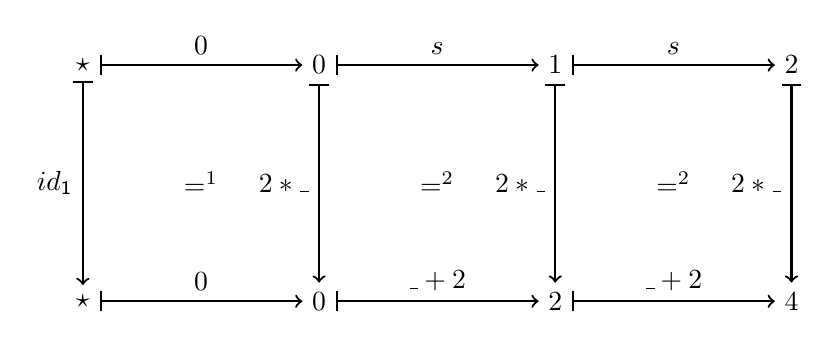
\begin{tikzpicture}
\node (s) at (0, 1) {$\star$};
\node (s') at (0, -2) {$\star$};
\node (f1) at (1.5, -0.5) {$=^1$};

\node (0) at (3, 1) {$0$};
\node (0') at (3, -2) {$0$};
\node (f1) at (4.5, -0.5) {$=^2$};

\node (1) at (6, 1) {$1$};
\node (1') at (6, -2) {$2$};
\node (f1) at (7.5, -0.5) {$=^2$};

\node (2) at (9, 1) {$2$};
\node (2') at (9, -2) {$4$};

\tikzset{mystyle/.style={|->,thick}};  
\path (s) edge [mystyle] node[above]{$0$} (0);
\path (0) edge [mystyle] node[above]{$s$} (1);
\path (1) edge [mystyle] node[above]{$s$} (2);

\path (s) edge[mystyle] node[left]{$id_{\mathsf 1}$} (s');
\path (0) edge[mystyle] node[left]{$2 * \_$} (0');
\path (1) edge[mystyle] node[left]{$2 * \_$} (1');
\path (2) edge[mystyle] node[left]{$2 * \_$} (2');

\path (s') edge [mystyle] node[above]{$0$} (0');
\path (0') edge [mystyle] node[above]{$\_ + 2$} (1');
\path (1') edge [mystyle] node[above]{$\_ + 2$} (2');
\end{tikzpicture}
\end{center}
$=^1$ is given by the base case in our definition (Figure 1) and $=^2$ is given by the induction step (Figure 2).
So $2 * 2 = 4$.
\end{example}

\section{Abstraction step : describe an algebra as a \textit{single} arrow}
A signature $\Sigma$ corresponds to a (type) functor $T_\Sigma : \mathsf{Set} \to \mathsf{Set}$. A $\Sigma$-\textit{algebra} $\ca$ with carrier set $A$, corresponds to a map $\alpha : T_\Sigma(A) \to A$. \truls{Need more? Didn't write down the general definition. Could invent it, but not completely sure where I'd stick the parameters if there are any.}

\section{Categories}
We abstract.

\subsection{$\mathsf{Alg}(T_\Sigma) \cong \mathsf{Alg}(\Sigma)$}

Each $T_\Sigma$-algebra $(\alpha, A)$ defines a $\Sigma$-algebra $\ca_\alpha$ with carrier $A$ and operations $op^{\ca_\alpha} = x_i;\alpha$. 

\begin{proposition} $\ca_{\alpha_\ca} = \ca$
\end{proposition}

\begin{proof} 1 and 2
\begin{enumerate}
\item $\ca \mapsto (\alpha_\ca, A) \mapsto \ca_{\alpha_\ca} = \ca$
\item $(\alpha, A) \mapsto \ca_\alpha \mapsto (\alpha_{\ca_\alpha}, A) = (\alpha, A)$
\end{enumerate}

\end{proof}

\subsection{Algebras and Limits}
Let $T$ be an endofunctor in category $\mathbb C$. Then $Alg(T)$ is the category of algebras of that type. 

\begin{proposition} $\mathsf{Alg}(T)$ inherits all limits from $\mathbb C$.
\end{proposition}

Limits in $\mathsf{Alg}(T)$ are constructed by the limits on the \textit{carrier} from $\mathbb C$.

\begin{example} We illustrate the previous proposition with \textit{product}.

\begin{figure}[ht]
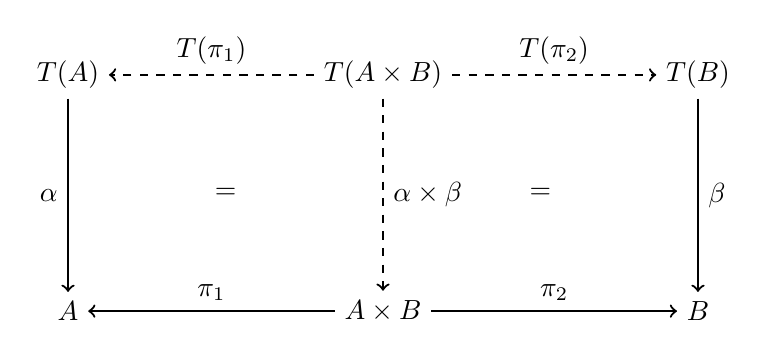
\begin{tikzpicture}
\node (tab) at (0, 0) {$T(A \times B)$};
\node (ta) at (-4, 0) {$T(A)$};
\node (tb) at (4, 0) {$T(B)$};

\node (ab) at (0, -3) {$A \times B$};
\node (a) at (-4, -3) {$A$};
\node (b) at (4, -3) {$B$};

\node (eq1) at (2, -1.5) {$=$};
\node (eq2) at (-2, -1.5) {$=$};

\tikzset{mystyle/.style={->,thick,dashed}};  
\path (tab) edge [mystyle] node[above]{$T(\pi_1)$} (ta);
\path (tab) edge [mystyle] node[above]{$T(\pi_2)$} (tb);
\path (tab) edge[mystyle] node[right]{$\alpha \times \beta$} (ab);

\tikzset{mystyle/.style={->,thick}};  
\path (ab) edge [mystyle] node[above]{$\pi_1$} (a);
\path (ab) edge [mystyle] node[above]{$\pi_2$} (b);
\path (ta) edge[mystyle] node[left]{$\alpha$} (a);
\path (tb) edge[mystyle] node[right]{$\beta$} (b);
\end{tikzpicture}
\caption{$\alpha \times \beta ~:=~ \langle T(\pi_1);\alpha, T(\pi_2);\beta \rangle$ }
\end{figure}
\end{example}

(``limits/products are easy for algebras, \textit{because} the carrier is isolated on the RHS.'')

\begin{proposition} If $\mathbb C$ is a category with (an?) initial object and colimits of ascending chains and $T$ is an endofunctor in $\mathbb C$ which preserves colimits of ascending chains, then the category $\mathsf{Alg}(T)$ has (an?) initial object.
\end{proposition}

\section{Coalgebras $\cong$ systems with ``next-state semantics''}
Here are some coalgebras, which are of the form $A \to T(A)$ (turn the arrow). 

\begin{example} Examples of coalgebras. (Exercise: Describe the systems with words.)
\begin{enumerate}
\item $T(X) = X$, hence $\alpha : X \to T(X)$.
\item $T(X) = X + \mathsf 1$
\item $T(X) = X \times A$ ($A$ is just a parameter (e.g., a set of symbols))
\item $T(X) = X \times A + \mathsf 1$
\item $T(X) = [A \to X]$ ($[A \to X] \cong X^A$ (maps from $A$ to $X$))
\item $T(X) = \wp(X)$
\end{enumerate}
\end{example}

The category of $T$-coalgebras are denoted $\mathsf{CAlg}(T)$.

\begin{proposition} Let $T$ be an endofuctor in $\mathbb C$. $\mathsf{CAlg}(T)$ inherits all \textit{colimits} from $\mathbb C$.
\end{proposition}

\begin{example}The example of \textit{sum} would be basically the same the the example of \textit{product} above, but with the arrows going the other way.
\end{example}

\begin{example}Let $T(X) = X$. Coalgebras in $\mathsf{CAlg}(T)$ are of the form $\alpha : X \to X$. Given a state $x \in X$, we ``transition'' deterministically and unabiguously into the next state $\alpha(x) \in X$.
\begin{figure}[ht]
\begin{minipage}[b]{0.3\linewidth}
\begin{center}
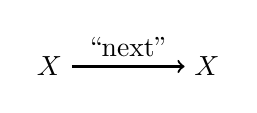
\begin{tikzpicture}
\node (xl) at (0, 0) {$X$};
\node (xr) at (2, 0) {$X$};

\tikzset{mystyle/.style={->,thick}};  
\path (xl) edge[mystyle] node[above]{``next''} (xr);
\end{tikzpicture}
\end{center}
\caption{``Shape''}
\end{minipage}
\begin{minipage}[b]{0.3\linewidth}
\begin{center}
\begin{tikzpicture}[scale=0.7]
\node (x1) at (0, 0) {$\cdot$};
\node (x2) at (-1, 1) {$\cdot$};
\node (x3) at (-1, -1) {$\cdot$};
\node (x4) at (-2.5, -1) {$\cdots$};
\node (x5) at (-2.5, 1) {$\cdots$};
\node (x6) at (1.5, 0) {$\cdots$};

\tikzset{mystyle/.style={->,thick}};  
\path (x1) edge[mystyle] node[]{} (x6);

\path (x2) edge[mystyle] node[above]{} (x1);
\path (x5) edge[mystyle] node[above]{} (x2);

\path (x3) edge[mystyle] node[above]{} (x1);
\path (x4) edge[mystyle] node[above]{} (x3);
\end{tikzpicture}
\end{center}
\caption{\\Arbitrary}
\end{minipage}
\begin{minipage}[b]{0.3\linewidth}
\begin{center}
\begin{tikzpicture}
\node (x) at (0, 0) {$\cdot$};

\tikzset{mystyle/.style={->,thick}};  
\path (x.0) edge[mystyle] node[bend right]{} (x.90);
\end{tikzpicture}
\end{center}
\caption{\\Final}
\end{minipage}
\end{figure}
\end{example}
\truls{The ``Final'' one above should just be a reflexive point. Don't know tikzpicture well enough to do that.}

\subsection{Discussion}
Recall (and extrapolate): 
\begin{itemize}
\item initial algebra $\cong$ induction. Dually, final coalgebra $\cong$ coinduction.
\item elements of initial algebra: (ground) terms; elements of final coalgebra: process/language/observable behaviour of systems.
\item ``final'' $\rightsquigarrow$ ``identify (``collapse'') as much as possible''. Need a way to ``avoid trivial collapse'': two elements/states in the final coalgebra are different if they can be distinguished by \textit{observations}. (Think \textit{bisimulation}!)
\end{itemize}

\subsection{Constructing the final coalgebra.} But first recall:
\subsubsection{Constructing the initial algebra $T^*(\mathcal I)$}
For simplicity assume that $T : \mathsf{Set} \to \mathsf{Set}$. Then $\mathcal I = \emptyset$. We start with an empty set of terms $\emptyset$, then construct all terms of ``complexity'' at most 1, then all terms of ``complexity'' at most 2, and so on. We collect these in the colimit, the set of all (reachable/ground) terms. See Figure (number).

\begin{figure}[ht]
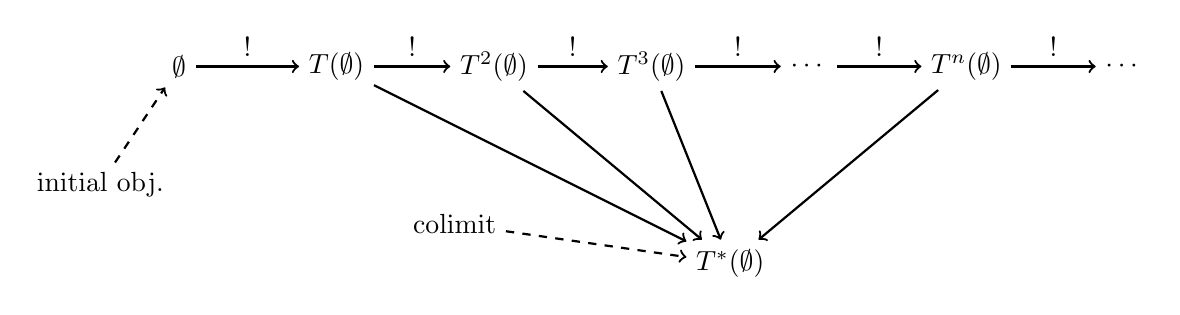
\begin{tikzpicture}
\node (01) at (0, 0) {$\emptyset$};
\node (02) at (2, 0) {$T(\emptyset)$};
\node (03) at (4, 0) {$T^2(\emptyset)$};
\node (04) at (6, 0) {$T^3(\emptyset)$};
\node (05) at (8, 0) {$\cdots$};
\node (06) at (10, 0) {$T^n(\emptyset)$};
\node (07) at (12, 0) {$\cdots$};

\node (star) at (7, -2.5) {$T^*(\emptyset)$};

\node (t1) at (-1, -1.5) {initial obj.};
\node (t2) at (3.5, -2) {colimit};

\tikzset{mystyle/.style={->,thick}};  
\path (01) edge[mystyle] node[above]{!} (02);
\path (02) edge[mystyle] node[above]{!} (03);
\path (03) edge[mystyle] node[above]{!} (04);
\path (04) edge[mystyle] node[above]{!} (05);
\path (05) edge[mystyle] node[above]{!} (06);
\path (06) edge[mystyle] node[above]{!} (07);

\path (02) edge[mystyle] node[above]{} (star);
\path (03) edge[mystyle] node[above]{} (star);
\path (04) edge[mystyle] node[above]{} (star);
\path (06) edge[mystyle] node[above]{} (star);

\tikzset{mystyle/.style={->,thick,dashed}};  
\path (t1) edge[mystyle] node[above, bend left]{} (01);
\path (t2) edge[mystyle] node[above, bend left]{} (star);
\end{tikzpicture}
\caption{Constructing the initial algebra.}
\end{figure}

Now, to construct the final coalgebra:\\

\begin{figure}[ht]
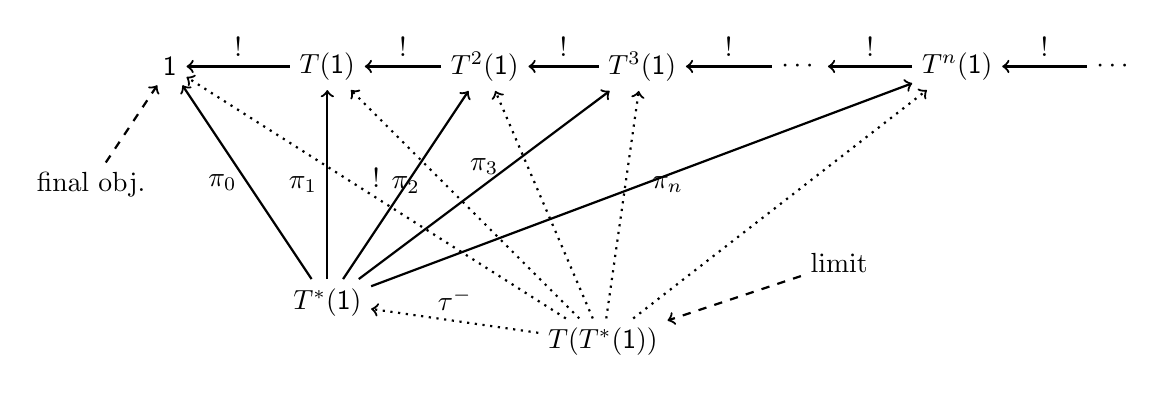
\begin{tikzpicture}
\node (01) at (0, 0) {$\mathsf 1$};
\node (02) at (2, 0) {$T(\mathsf 1)$};
\node (03) at (4, 0) {$T^2(\mathsf 1)$};
\node (04) at (6, 0) {$T^3(\mathsf 1)$};
\node (05) at (8, 0) {$\cdots$};
\node (06) at (10, 0) {$T^n(\mathsf 1)$};
\node (07) at (12, 0) {$\cdots$};

\node (star1) at (2, -3) {$T^*(\mathsf 1)$};
\node (star2) at (5.5, -3.5) {$T(T^*(\mathsf 1))$};

\node (t1) at (-1, -1.5) {final obj.};
\node (t2) at (8.5, -2.5) {limit};

\tikzset{mystyle/.style={->,thick}};  
\path (02) edge[mystyle] node[above]{!} (01);
\path (03) edge[mystyle] node[above]{!} (02);
\path (04) edge[mystyle] node[above]{!} (03);
\path (05) edge[mystyle] node[above]{!} (04);
\path (06) edge[mystyle] node[above]{!} (05);
\path (07) edge[mystyle] node[above]{!} (06);

\path (star1) edge[mystyle] node[left]{$\pi_0$} (01);
\path (star1) edge[mystyle] node[left]{$\pi_1$} (02);
\path (star1) edge[mystyle] node[]{$\pi_2$} (03);
\path (star1) edge[mystyle] node[above]{$\pi_3$} (04);
\path (star1) edge[mystyle] node[right]{$\pi_n$} (06);

\tikzset{mystyle/.style={->,thick,dotted}};  
\path (star2) edge[mystyle] node[above]{!} (01);
\path (star2) edge[mystyle] node[above]{} (02);
\path (star2) edge[mystyle] node[above]{} (03);
\path (star2) edge[mystyle] node[above]{} (04);
\path (star2) edge[mystyle] node[above]{} (06);

\path (star2) edge[mystyle] node[above]{$\tau^-$} (star1);

\tikzset{mystyle/.style={->,thick,dashed}};  
\path (t1) edge[mystyle] node[above, bend left]{} (01);
\path (t2) edge[mystyle] node[above, bend left]{} (star2);
\end{tikzpicture}
\caption{Constructing the initial algebra.}
\end{figure}

\truls{I don't know. I don't get it anymore.}

There is a unique $\tau^- : T(T^*(\mathsf 1)) \to T^*(\mathsf 1)$ such that $\tau^-;\pi_i = T(\pi_{i - 1})$. 

We still need $\tau : T_*(\mathsf 1) \to T(T_*(\mathsf 1))$. 

\truls{Could someone descripbe this process?}

\end{document}
